\section{Vòng đời mô hình AI và cơ chế huấn luyện}

\subsection{Tổng quan vòng đời mô hình}
Trong quá trình xây dựng dự án, mô hình không được tổ chức như một artifact tĩnh chỉ huấn luyện một lần rồi sử dụng cố định mà toàn bộ luồng xử lý đã được thiết kế theo tư duy vòng đời mô hình, trong đó dữ liệu được cập nhật, mô hình được huấn luyện lại, kết quả được đánh giá, phiên bản mới được lưu trữ, phiên bản đang hoạt động được lựa chọn, và cuối cùng mô hình mới được đưa vào phục vụ suy luận. Cách tổ chức này giúp phần AI gắn trực tiếp với vận hành của ứng dụng thay vì tồn tại như một thành phần tách rời.

\begin{figure}[htbp]
    \centering
    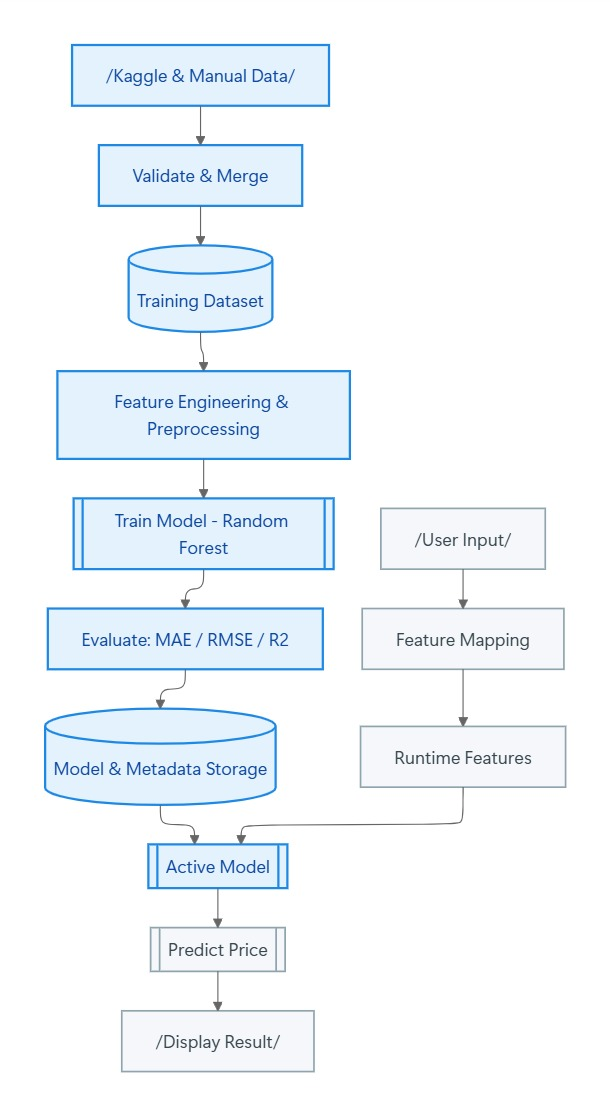
\includegraphics[width=0.80\textwidth,height=0.68\textheight,keepaspectratio]{chapters/AI_pineline.jpg}
    \caption{Sơ đồ luồng AI pipeline của hệ thống}
    \label{fig:ai-pipeline-mermaid}
\end{figure}

Với pipeline hiện tại, dữ liệu đầu vào được lấy từ tập Kaggle và có thể được mở rộng bằng các bản ghi thêm thủ công hoặc sinh tự động bởi hệ thống nhằm tăng độ phong phú của tập huấn luyện. Sau bước kiểm tra schema, dữ liệu được hợp nhất và lưu lại thành tập làm việc chung. Từ tập này, pipeline tiếp tục thực hiện tách train/test, tiền xử lý đặc trưng, huấn luyện mô hình Random Forest, tính các độ đo đánh giá, lưu artifact, lưu metadata và cập nhật phiên bản đang hoạt động.

Ở nhánh suy luận, dữ liệu do người dùng nhập từ giao diện không được đưa trực tiếp vào mô hình. Thay vào đó, đầu vào được ánh xạ qua catalog thiết bị và được dựng lại đúng cấu trúc đặc trưng mà mô hình đã dùng trong quá trình huấn luyện. Cách tổ chức này nhằm nâng cao trải nghiệm người dùng: nếu buộc người dùng nhập đầy đủ toàn bộ các đặc trưng như trong tập huấn luyện thì biểu mẫu sẽ rất dài và khó sử dụng. Với hướng tiếp cận hiện tại, người dùng chỉ cần cung cấp một số thông tin bề mặt như model, tình trạng pin hoặc thời gian sử dụng, còn hệ thống sẽ suy ra và điền tiếp các thông số phần cứng liên quan từ catalog thiết bị đã xây dựng sẵn. Nhờ đó, giao diện vẫn gọn, dễ thao tác và gần hơn với cách người dùng thực tế mô tả một chiếc điện thoại cần định giá.

\subsection{Cơ chế huấn luyện}

Ứng dụng cho phép người vận hành có thể nhập các siêu tham số chính của mô hình, đồng thời bật chế độ chọn feature tùy biến cho từng lần huấn luyện. Cụ thể, hệ thống cho phép giữ bộ feature mặc định hoặc đánh dấu lại từng biến đầu vào như brand, RAM, storage, battery, screen size, camera, release year, days used và một số biến mở rộng khác. Nhờ đó, dashboard không chỉ phục vụ thao tác train model đơn thuần mà còn hỗ trợ so sánh nhiều cấu hình đầu vào khác nhau ngay trong cùng một môi trường vận hành.

\blockparagraph{Phân tích kỹ thuật tối ưu hóa trong quá trình huấn luyện}

Mô hình lõi được chọn cho bài toán là Random Forest Regressor. Với lựa chọn này, phần ``tối ưu hóa'' trong quá trình huấn luyện không được hiểu theo nghĩa cập nhật trọng số bằng gradient descent như trong mạng nơ-ron, mà được hiểu theo nghĩa lựa chọn cấu trúc cây và điều chỉnh siêu tham số để đạt khả năng tổng quát hóa tốt trên dữ liệu chưa thấy.

Nhóm tham số điều chỉnh chính được đưa ra cho quá trình huấn luyện gồm các siêu tham số của mô hình và cả lựa chọn tập feature đầu vào:

\begin{itemize}
    \item \texttt{n\_estimators}: số cây trong rừng.
    \item \texttt{max\_depth}: độ sâu cực đại của mỗi cây.
    \item \texttt{min\_samples\_split}: số mẫu tối thiểu để một nút được phép tách.
    \item \texttt{min\_samples\_leaf}: số mẫu tối thiểu ở một nút lá.
    \item \texttt{features}: tập đặc trưng được chọn cho lần huấn luyện, có thể dùng bộ mặc định hoặc tùy chỉnh trực tiếp trên dashboard.
\end{itemize}

Trong quá trình thiết kế, các tham số này được xem như công cụ kiểm soát trực tiếp cả độ phức tạp của mô hình lẫn phạm vi thông tin đầu vào mà mô hình được phép sử dụng. Khi tăng số cây, dự đoán thường ổn định hơn nhưng chi phí huấn luyện và suy luận cũng tăng theo. Khi cho phép cây quá sâu hoặc lá quá nhỏ, mô hình có xu hướng bám sát dữ liệu huấn luyện hơn mức cần thiết. Ở chiều ngược lại, việc thêm hoặc bớt feature cũng làm thay đổi khả năng biểu đạt của mô hình và mức độ rủi ro leakage. Vì vậy, quá trình huấn luyện trong hệ thống được thiết kế theo hướng cho phép thử nghiệm linh hoạt nhiều cấu hình, nhưng vẫn giữ một lõi xử lý thống nhất để bảo đảm tính nhất quán giữa các lần train.

\subsection{Kiểm soát chất lượng mô hình và tính hợp lệ đặc trưng}

\blockparagraph{Kiểm soát overfitting}

Trong hệ thống hiện tại, kiểm soát overfitting được thực hiện bằng các cơ chế phù hợp với mô hình cây thay vì vay mượn các kỹ thuật của deep learning. Trọng tâm nằm ở việc giảm phương sai của ensemble, giới hạn độ phức tạp của từng cây và tránh để mô hình hấp thụ các tín hiệu quá gần với biến mục tiêu.

\begin{enumerate}[label=\arabic*.]
    \item \textbf{Ensemble averaging:} lấy trung bình trên nhiều cây để làm mượt dự đoán và giảm phương sai tổng thể.
    \item \textbf{Giới hạn độ phức tạp cây:} dùng \texttt{max\_depth}, \texttt{min\_samples\_split} và \texttt{min\_samples\_leaf} để ngăn cây phát triển quá mức.
    \item \textbf{Kiểm soát phạm vi feature:} cho phép chọn tập đặc trưng huấn luyện nhưng vẫn giữ một bộ mặc định gọn, tránh mở rộng đầu vào không kiểm soát.
\end{enumerate}

\blockparagraph{Tính hợp lệ của dữ liệu và đặc trưng}

Ngoài overfitting theo nghĩa mô hình, hệ thống còn kiểm soát chất lượng dự đoán ở lớp dữ liệu và đặc trưng. Các bước như kiểm tra schema, chuẩn hóa bản ghi và loại bỏ biến có nguy cơ leakage được xem là điều kiện bắt buộc để bảo đảm dữ liệu train và dữ liệu suy luận đều phản ánh đúng tín hiệu nghiệp vụ hợp lệ.

\blockparagraph{Feature validity và target leakage}

Biến \texttt{normalized\_new\_price} không được đưa vào tập mặc định vì có tương quan quá mạnh với giá cần dự đoán. Về mặt kiến trúc, đây là quyết định thuộc \textit{data/feature validity}: mục tiêu là tránh một mô hình cho kết quả đẹp trên tập đánh giá nhưng phụ thuộc vào thông tin không bền vững hoặc khó thu thập ở thời điểm suy luận thực tế.

\subsection{Quản trị vòng đời mô hình và vận hành suy luận}

Theo phân lớp chuẩn của ML system, toàn bộ các nội dung như metadata, versioning, chọn active model, inference consistency hay fallback runtime đều thuộc \textit{model lifecycle} và \textit{inference serving}.

\blockparagraph{Metadata huấn luyện}

Sau mỗi lần train, hệ thống lưu kèm \texttt{metadata.json} bên cạnh \texttt{model.pkl}. Metadata ghi nhận version, tập feature, target, chỉ số MAE/RMSE/$R^2$, siêu tham số và thời điểm huấn luyện; nhờ đó mỗi artifact có đủ ngữ cảnh để so sánh, truy vết và giải thích quyết định chọn mô hình.

\blockparagraph{Versioning mô hình}

Các phiên bản được tổ chức theo thư mục \texttt{app/model\_versions/v1}, \texttt{v2}, \ldots, và mỗi lần train mới tạo ra một version độc lập thay vì ghi đè artifact cũ. Cấu trúc này thuộc lớp \textit{model lifecycle management}, vì chức năng chính của nó là bảo toàn lịch sử, hỗ trợ rollback và cho phép so sánh giữa các lần huấn luyện.

\blockparagraph{Chọn active model}

Một model chỉ đi vào phục vụ suy luận khi được đánh dấu là \texttt{active\_model\_version} trong \texttt{app\_settings.json}. Cơ chế này tách quyết định vận hành khỏi mã nguồn ứng dụng, cho phép đổi model đang phục vụ như một thao tác quản trị thay vì một thay đổi logic trong pipeline.

\blockparagraph{Tính nhất quán của suy luận}

Ở thời điểm runtime, hàm \texttt{predict()} đọc lại cấu trúc đặc trưng đã được lưu cùng preprocessor hoặc regressor để dựng đúng thứ tự cột đầu vào. Đây là cơ chế \textit{inference consistency}: mục tiêu là bảo đảm model luôn nhận đúng schema mà version tương ứng đã dùng trong quá trình huấn luyện.

\blockparagraph{Cơ chế fallback}

Khi không nạp được bất kỳ artifact hợp lệ nào, hệ thống chuyển sang \texttt{\_mock\_predict()} để duy trì khả năng phản hồi tối thiểu. Về mặt kiến trúc, đây là một biện pháp \textit{runtime safety}, giúp ứng dụng không dừng hoàn toàn trong các tình huống lỗi artifact, demo hoặc kiểm thử giao diện.

\blockparagraph{Mức sẵn sàng vận hành}

Ở phạm vi hiện tại, hệ thống đã bao quát được một vòng đời vận hành khép kín: huấn luyện, lưu version, chọn active model và phục vụ suy luận trong cùng một ứng dụng. Tuy nhiên, nếu nâng lên production đầy đủ, cần bổ sung thêm các lớp như audit log, monitoring, kiểm soát đồng thời, backup artifact và quản trị lỗi ở mức dịch vụ.

